
\chapter{Characterization of Building Use, Performance, and Operations}
\label{sec:characterization}

Visualization of temporal features on their own is a means of understanding the range of values of the various phenomenon across a time range. This situation gives an analyst the basis to begin understanding what discriminates a building based on different objectives. The next step is to utilize the features to predict whether a building falls into a particular category and test the importance of various elements in making that prediction. Understanding which features are most characteristic to a particular objective is the fundamental tenet of this study. In this section, three classification objectives are tested: 

\begin{enumerate}
\item Principle Building Use - The primary use of the building is designated for the principal activity conducted by percentage of space designated for that activity. It is rare for a building to be devoted specifically to a single task, and mixed-use buildings pose a specific challenge to prediction.
\item Performance Class - Each building is assigned to a particular performance class according to whether its area-normalized consumption in the bottom, middle, or top 33\% percentiles within its principle building use-type class.
\item General Operation Strategy - Buildings that are controlled by the same entity, such as those on a University campus, often have similar schedules, operating parameters, and use patterns. This objective tests to understand how distinct these differences are between different campuses.
\end{enumerate}

\section{Principal Building Use}
\label{sec:buildinguse}

The first scenario investigated is the characterization of primary building use type. The goal of this effort is to quantify what temporal behavior \emph{is most characteristic in a building being used for a certain purpose}. For example, what makes the electrical consumption patterns of an office building unique as compared to other purposes such as a convenience store, airport, or laboratory. This objective is necessary to understand who are the \emph{peers} of a building. Whatever category a building is assigned determines what benchmark is used to determine the performance level of a building. The EnergyStar Portfolio Manager is the most common benchmarking platform in the United States and the first step in its evaluation is identifying the property type. There are 80 \emph{property types} in portfolio manager and each one is devoted to a particular primary building use type. Twenty-one of those property types are available for submission to achieve a 1-100 ENERGYSTAR score in the United States. These property types are seen in Figure \ref{fig:energystarbuildings}.

\begin{figure}[ht!]
\begin{center}
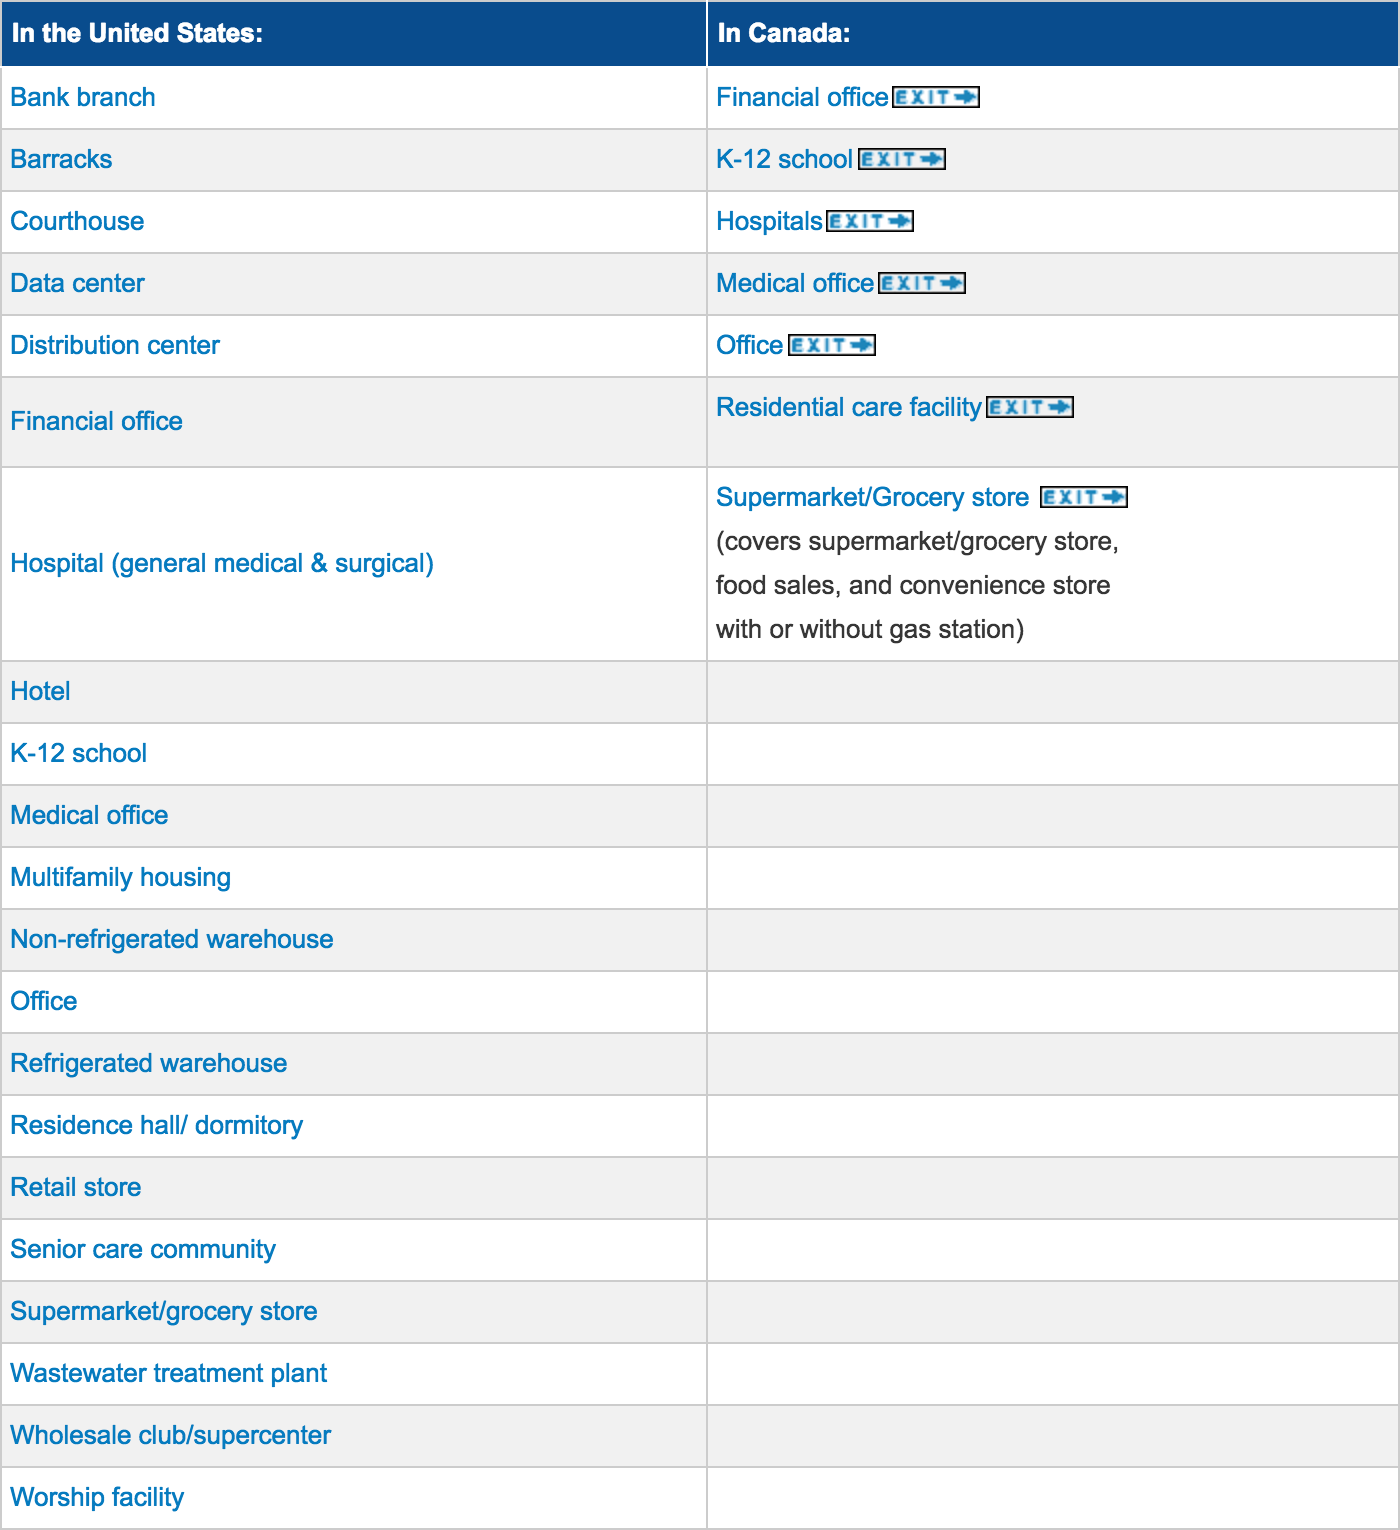
\includegraphics[width=0.7\columnwidth]{figures/enegystar_buildingtypes/enegystar_buildingtypes}
\caption{{EnergyStar building use-types available for 1-100 rating (from \url{https://www.energystar.gov/})
\label{fig:energystarbuildings}%
}}
\end{center}
\end{figure}

Allocation of the primary use type of a building is often considered a trivial activity when analyzed from a smaller set of buildings. As the number of building being analyzed grows, so does the complexity of space use evaluation. The use of buildings changes over time and these changes are not always documented. In several of the case studies, this topic was discussed and highlighted as an issue concerning benchmarking a building.\\
\\
Discriminatory features have already been visualized extensively in Sections \ref{sec:statisticsfeatures}-\ref{sec:patternbasedfeatures} and the differences between the primary use types are apparent in the overview heat maps of each feature. In this and the following sections, a quantification of the impact of each feature will be evaluated using a random forest model and its associated variable importance methods. Figure \ref{fig:use_classification} is the first such example of the output results of the classification model in predicting the building's primary use type using the temporal features created in this study. This visualization is a kind of error matrix, or confusion matrix, that illustrates the performance of a supervised classification algorithm. The \emph{y-axis} represents the correct label of each classification input and the \emph{x-axis} is the predicted label. An accurate classification would fall on the left-to-right diagonal of the grid. This grid is normalized according to the percentage of buildings within each class. The model was built using the scikit-learn Python library\footnote{http://scikit-learn.org/} with the number of estimators set to 100 and the minimum samples per leaf set to 2. The overall general accuracy of the model is 67.8\% as compared to a baseline model of 22.2\%. The baseline model using a stratified strategy in which categories are chosen randomly based on the percentage of each class occurring in the training set. Based on the analysis, university dormitories and primary/secondary classrooms are the best-characterized use types overall with precisions of 92\% and 96\% respectively and accuracies of 74\% and 75\%. The office category is easy confused with university classrooms and laboratories. This situation is not surprising as many of these facilities are quite similar and uses within these categories often overlap. 

\begin{figure}[ht!]
\begin{center}
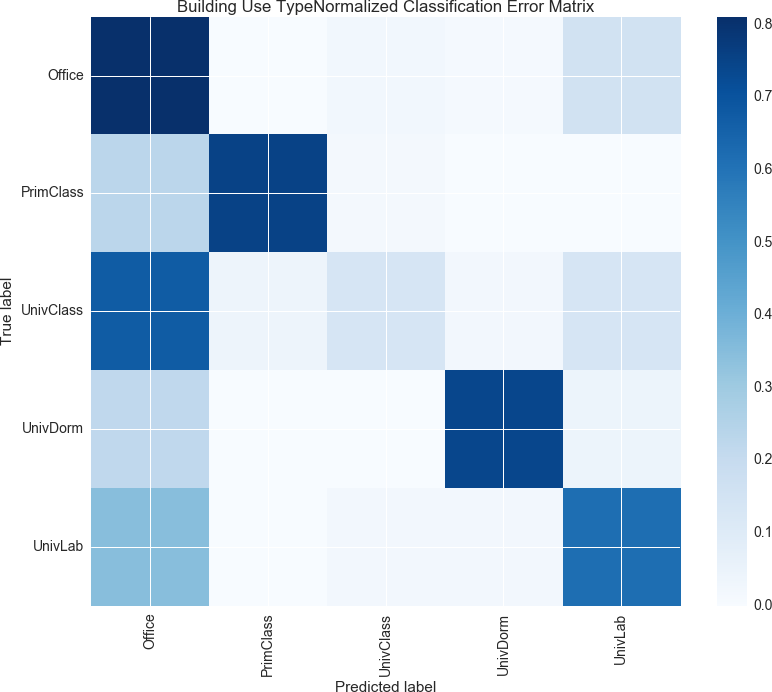
\includegraphics[width=1\columnwidth]{figures/ConfusionMatrixBuildingUseType/ConfusionMatrixBuildingUseType}
\caption{{Classification error matrix for prediction of building use type using a random forest model
\label{fig:use_classification}%
}}
\end{center}
\end{figure}

The most important features contributing to the accuracy of the classification model are found in Figure \ref{sec:featureimportance_usetype}. These features are ranked according to their importance in designating the difference between all of the building types. Three of the top fifteen most important features are from the \emph{stl} decomposition process. This fact shows the importance that normalized weekly patterns play in differentiation, in particular for dormitories. Eight of the fifteen are statistical metrics, either ratios or consumption statistics. The second highest variable importance is related to the correlation output from the loadshape model. And the remaining three variables pertain to the number of long-term breakouts, and thus, volatility.

\begin{figure}[ht!]
\begin{center}
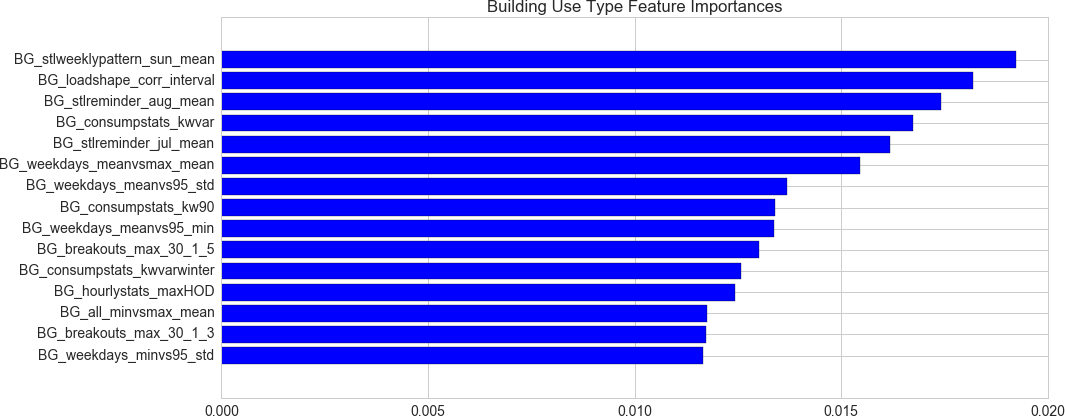
\includegraphics[width=1\columnwidth]{figures/FeatureImportanceBuildingUseType1/FeatureImportanceBuildingUseType1}
\caption{{Importance of features in prediction of building use type
\label{sec:featureimportance_usetype}%
}}
\end{center}
\end{figure}

\subsection{University Dormitory and Laboratory Comparison}
\label{sec:dormvslab}

The random forest classification model and variable importance metrics provide an indication of how the features characterize a building's use. A deeper investigation of the features with a comparison between two use types is useful to understand the characterization potential of various subsets of features. For this example, two building type classifications are compared that showed sharp distinction from each other in the random forest model: university laboratories and dormitories. For this comparison, the highly comparative time-series analysis (hctsa) code repository is used as a toolkit for analysis of the generated temporal features in this study \cite{Fulcher_2013}. This toolkit has various visualization tools that enable analysis of the predictive capabilities of temporal features. Figure \ref{fig:featurecluserting_dormvslabs} shows the top forty features in differentiating university laboratories and dormitories using a simple linear classifier model. These features are clustered according to their absolute correlation coefficients to understand how many unique sets of informative features are present. Groups of features in the same cluster are essentially giving the same type of information about the differences between a certain set of tested classes. In the case of laboratories and dormitories, there are eight sets of clusters giving information about this distinction. The first, fourth and fifth clusters contain a couple of breakout metrics representing volatility. The second and third clusters represent magnitudes of cooling energy and consumption statistics. The sixth cluster represents seasonal metrics. The seventh cluster is a collection of fourteen features that are highly correlated, with most being related to daily ratios and consumption-related metrics. The eighth and last cluster include fifteen features, several representing consumption metrics and ratios, but also several related to daily pattern frequencies.

% This toolkit includes a library of temporal features, however at this point in the analysis, only the features developed in this study are used.

%The first cluster (starting in the upper left corner of the confusion matrix) is a pair of breakout detection features measuring volatility over the long term. The next three clusters consist of a single feature; two of them describing hour-of-day metrics and one a daily pattern feature. The fifth cluster is a large group of eighteen features that are correlated with each other and all giving similar information regarding distinction. The most prominently distinctive features amongst this set are the ratio of mean and the 95th percentile. Most of the other features in this group are also daily statistics or consumption-focused metrics. The sixth cluster encompasses features related to the residuals \emph{stl} and \emph{eemeter} models. The seventh and eighth clusters are similar to the fifth cluster in having a large number of features related to daily ratios and patterns. The conclusion to be drawn from this analysis is that these two classifications are quite distinct mostly due to consumption magnitudes and the various daily load ratios in addition to several weekly and daily pattern-based features.

\begin{figure}[ht!]
\begin{center}
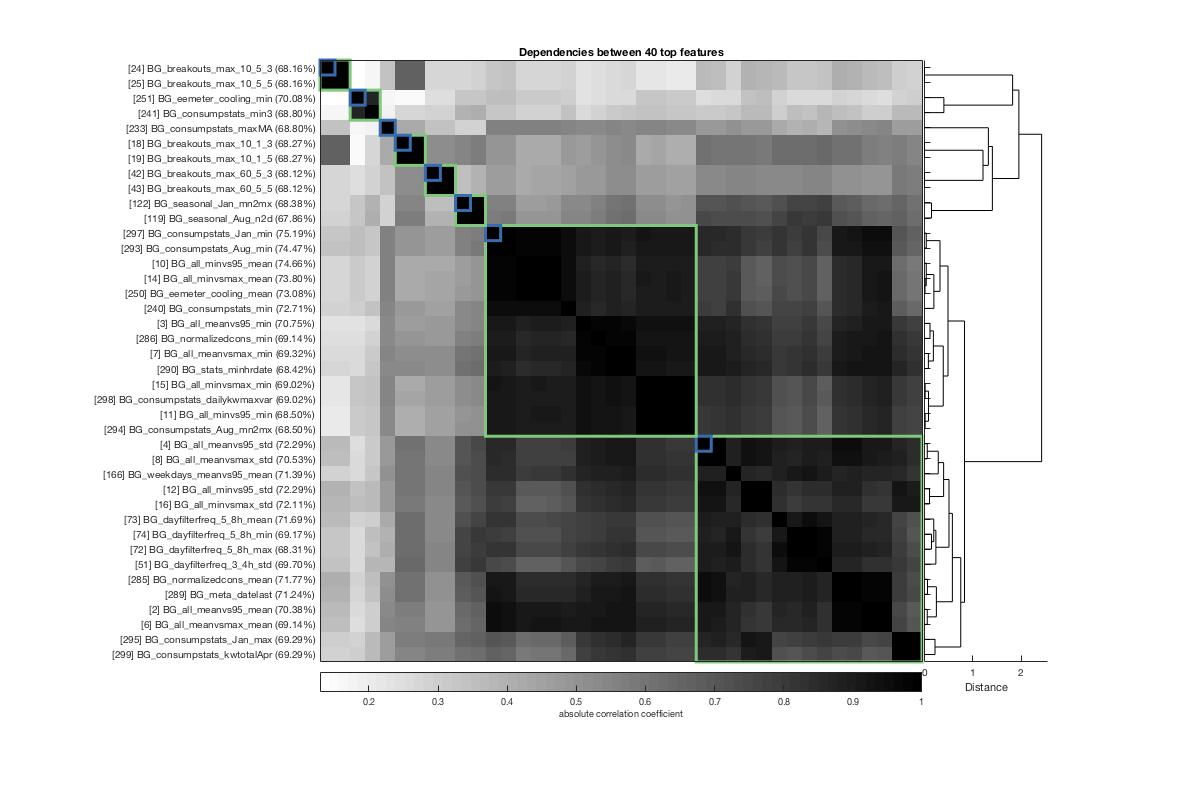
\includegraphics[width=1\columnwidth]{figures/Output_UnivDormVsClass_Top40/Output_UnivDormVsLab_Top40}
\caption{{Clustering of dominant features in the comparison of university dormitories and laboratories
\label{fig:featurecluserting_dormvslabs}%
}}
\end{center}
\end{figure}

Figure \ref{fig:topfivefeatures_dormvslab} illustrates the probability distributions of the top five differentiating features for distinguishing laboratories from dormitories. The probability density of each of the features is relatively similar in shape and distribution. This situation is because most of the features are from clusters seven and eight which are highly correlated within the cluster and between the clusters as well.

\begin{figure}[ht!]
\begin{center}
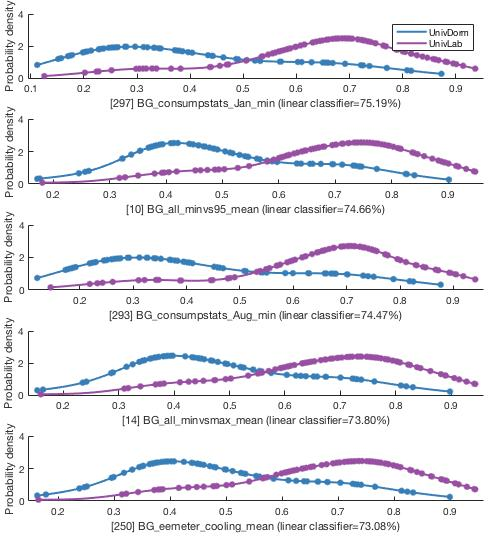
\includegraphics[width=0.7\columnwidth]{figures/Output_UnivDormVsLab_Features_1-5/Output_UnivDormVsLab_Features_1-5}
\caption{{Probability density distribution of top five features in characterizing the difference between university dormitories and laboratories
\label{fig:topfivefeatures_dormvslab}%
}}
\end{center}
\end{figure}

Figure \ref{sec:labsvsdorms_nullhypth} shows a distribution of the library of features on the data set compared to a benchmark of nulls generated by randomly selecting the class. This visualization indicates that there is a clear statistical difference in discriminating these two categories for a significant number of the input features. The real mean is approximately 62\%, while the null mean is slightly above 50\%. The ability to distinguish between these two classes is relatively high.

\begin{figure}[ht!]
\begin{center}
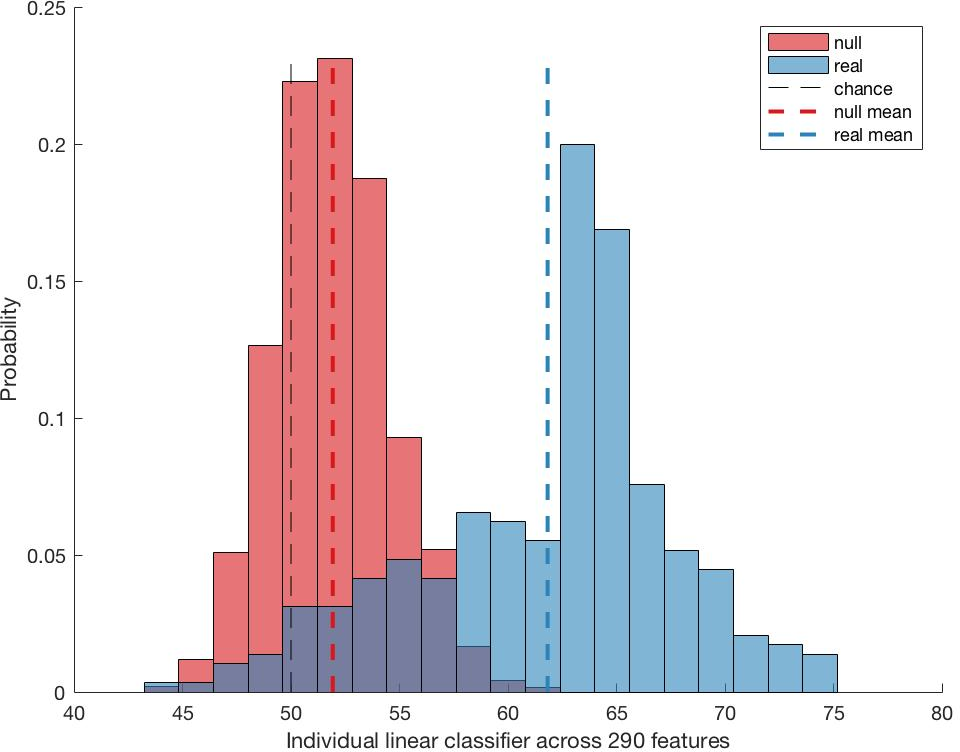
\includegraphics[width=0.7\columnwidth]{figures/Output_UnivDormVsLab_Dist/Output_UnivDormVsLab_Dist}
\caption{{Ability of temporal features to distinguish between dormitories and laboratories as compared to the null hypothesis
\label{sec:labsvsdorms_nullhypth}%
}}
\end{center}
\end{figure}

\subsection{Discussion with Campus Case Study Subjects}
\label{sec:buildinguseclassificationdiscussion}

Previously, an example of how to characterize building use type was illustrated using a random forest model and various feature importance techniques. In this subsection, a discussion is presented of how this sort of characterization can be useful in a practical setting. In the case study interviews, the topic of benchmarking of buildings was discussed. One of the issues presented to the operations teams was the concept of not having a complete understanding of the way the buildings on their campus were being used. For example, several of the campuses have a spreadsheet outlines various metadata about the facilities on campus. This worksheet, in many cases, includes the \emph{primary use type} of the building. It was found that this primary use type designation is often loosely based on information from when the building was constructed or through informal site survey. In other situations, the building has an accurate breakdown of all the sub-spaces in the building and approximately what the spaces are being used for. In these discussions, the idea was presented that building use type characterization could be used to determine automatically whether the labels within these spreadsheets aligned with the patterns of use characterization using the temporal feature extraction. This proposal was met some positive feedback, albeit there was a hesitation to confirm fully that this process would be entirely necessary if labor were directed to do the same task.\\
\\
Many of the case study subjects then were shown a series of graphics designed to tell the story of building use type characterization in an automated way. Figure \ref{fig:buildingusebreakdownforcasestudies} is the first graphic shown to the subjects. This figure illustrates several of the most easily understood temporal features and how they break down across the various building use types. This graphic was created using the data for a particular case study; therefore more separation between the classes exist than in the prediction of classes found in the previous section. Discussions using this graphic first centered around the first feature: \emph{Daily Magnitude per Area}. It was intuitive to most participants that a university laboratory has more and primary/secondary schools have less consumption per area than the other use types. It is more surprising, however, that certain building use types are characterized well by other features, such as a number of breakouts with primary/secondary schools and daily and weekly specificity with university dormitories.

% Grouping of characteristically similar buildings visualize and explore the \emph{phenotypes} of buildings. The objective of this section is focused on the identification of the primary modes in which in building use-type manifests itself and the identification of \emph{misfit} buildings or those that don't seem to act like they're supposed to.

\begin{figure}[ht!]
\begin{center}
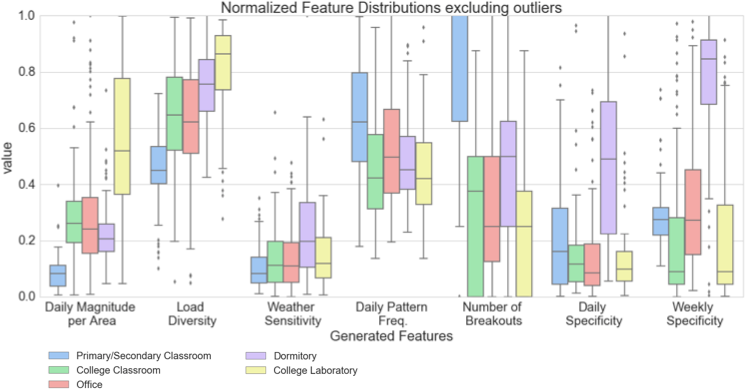
\includegraphics[width=0.98\columnwidth]{figures/buildingusecharacterization/buildingusecharacterization}
\caption{{Simplified breakdowns of general features according to building use type that were presented to case study subjects
\label{fig:buildingusebreakdownforcasestudies}%
}}
\end{center}
\end{figure}

After a discussion of how different use types of buildings are characterized using temporal features, the concept of misclassified buildings was introduced. Misclassification of buildings pertains to when the primary use type of the building doesn't match the temporal features of the electrical consumption, particularly the daily and weekly patterns of use. Figure \ref{fig:specificity_high} was designed to illustrate this concept. This figure contains a subset of the case study buildings within the office, university classroom, and university laboratory categories. The pattern specificity for offices, classrooms and laboratories were calculated for each building as shown in the first three columns of the graphic. They are clustered according to their similarity with red indicating low values and blue indicating high values. The column on the far right indicates the use type classification for each building. The laboratories are yellow, classrooms are blue, and offices are green. It can be seen that there are distinct clusters of building types and a few regions in which there is a mix of building use types in the final column. 

\begin{figure}[ht!]
\begin{center}
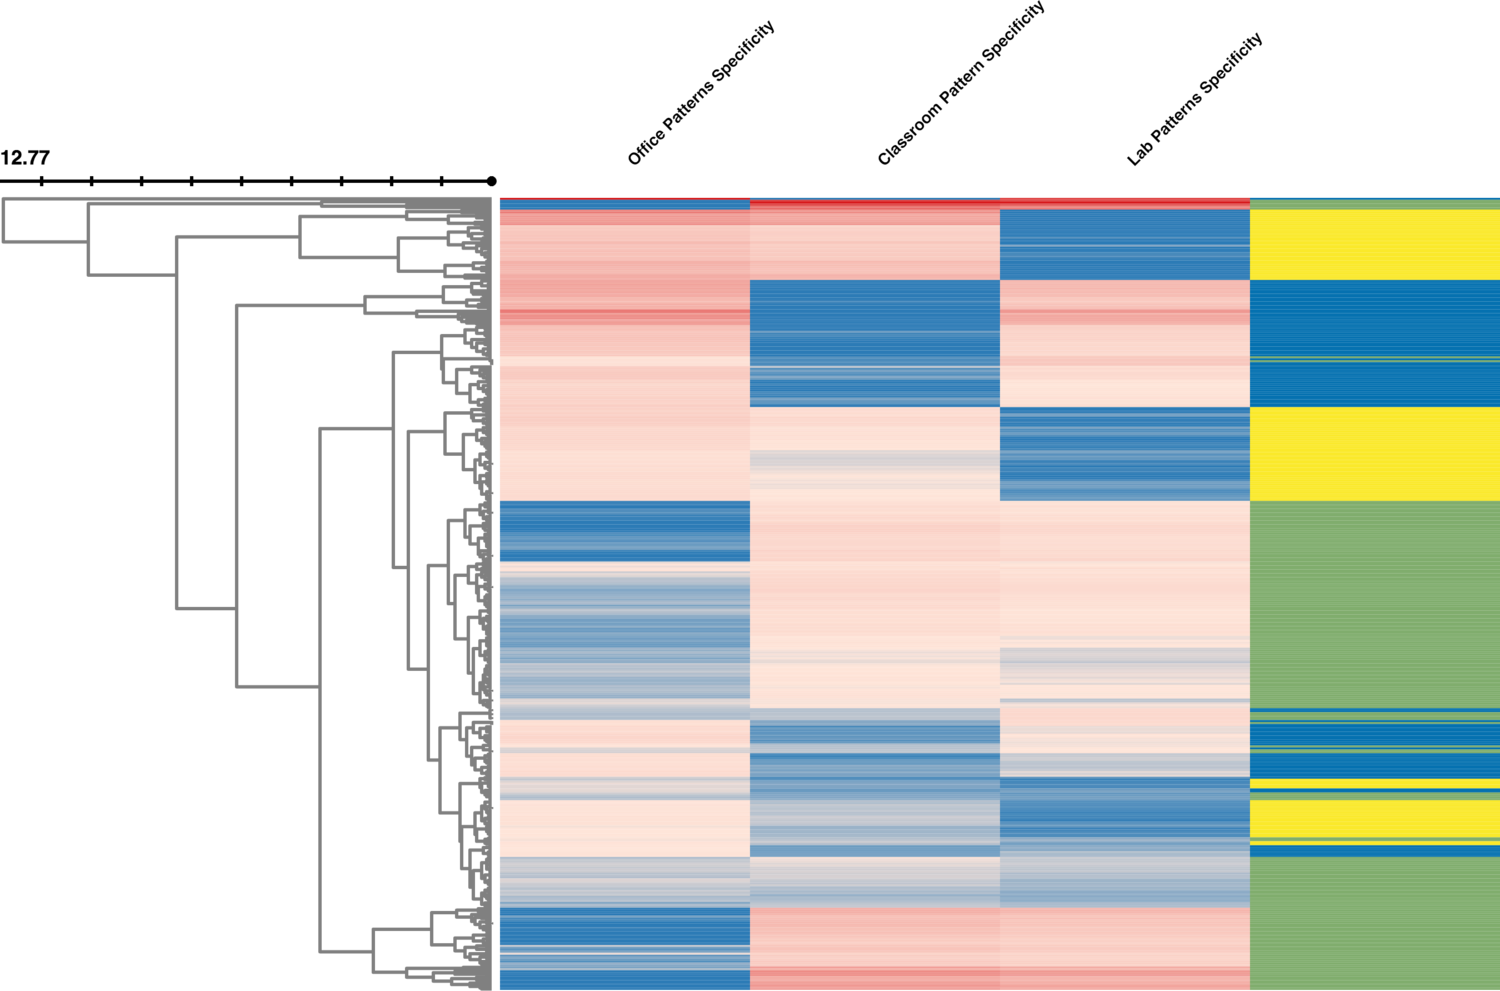
\includegraphics[width=1\columnwidth]{figures/clustering_weekly/clustering_weekly}
\caption{{Hierarchical clustering of buildings according to laboratory (yellow), office (green), and classroom (blue) specificity
\label{fig:specificity_high}%
}}
\end{center}
\end{figure}

Figure \ref{fig:decisiontree} shows the same diagram zoomed in on a certain subsection of a cluster that contains mostly buildings that identify as \emph{classrooms}. Interspersed amongst these classrooms are several buildings labeled as \emph{offices}. These offices can be potentially thought of as \emph{misfits} in that they are not members of more consistently homogeneous clusters. Discussions with members of the case study groups revealed that this information is \emph{interesting}, but immediately there wasn't a clear understanding of how this information would influence decision-making. It was suggested that this information could be used to supplement the results of the benchmarking process by giving more insight into potentially \emph{why} a building is not performing well within its class. The situation may actually be that the building is more a member of a different class and therefore may not be comparable to those particular \emph{peers}.

\begin{figure}[ht!]
\begin{center}
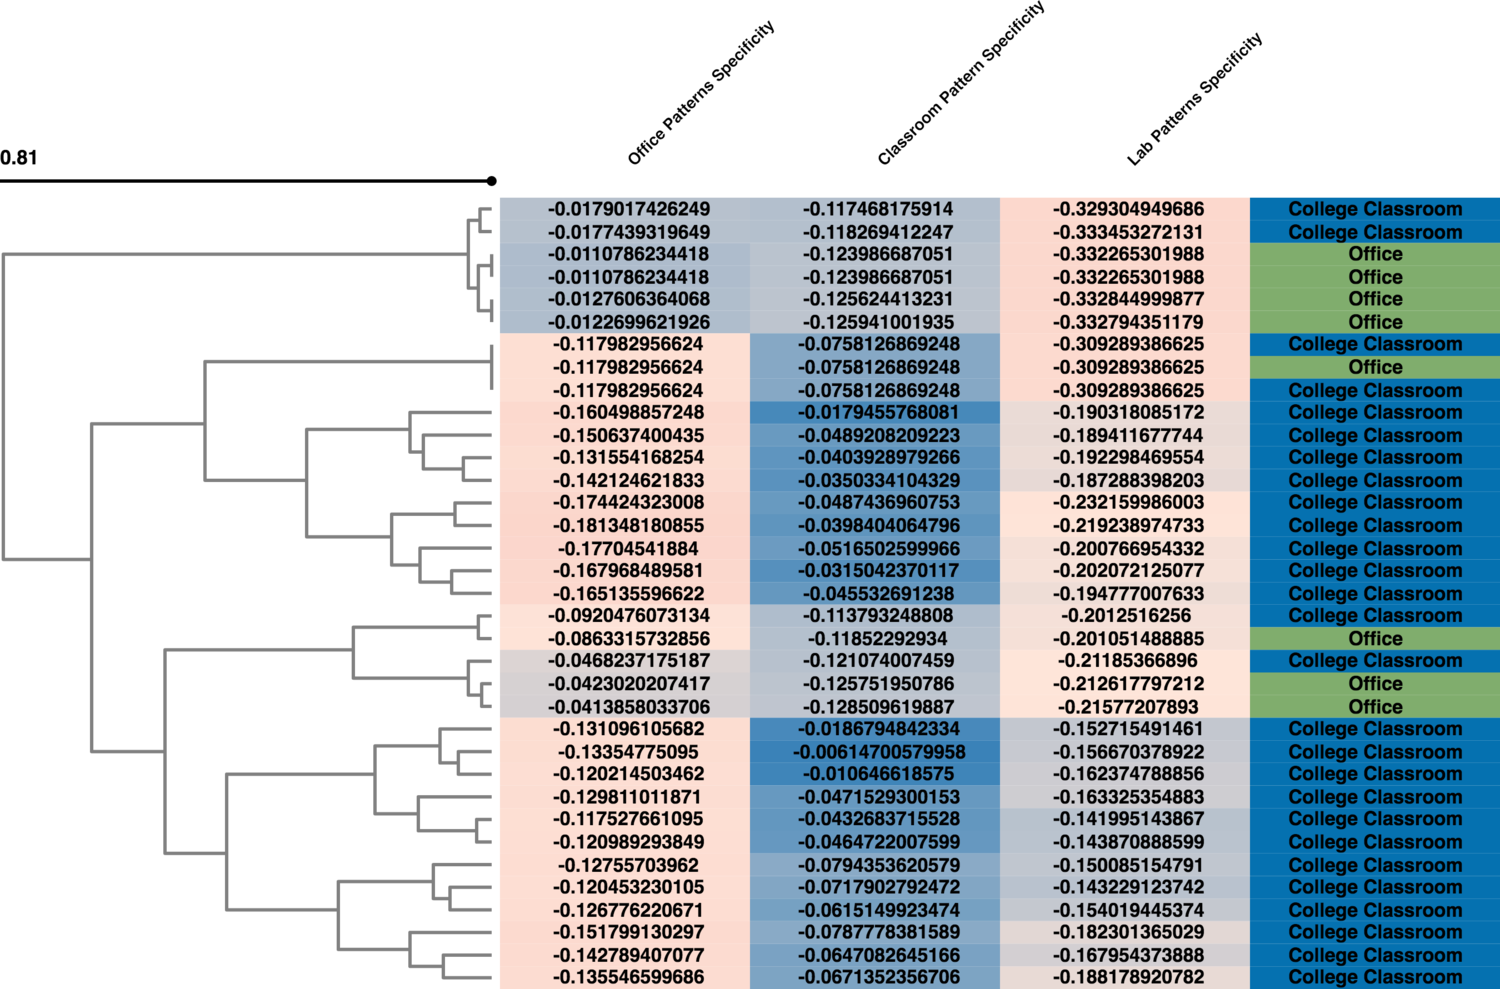
\includegraphics[width=1\columnwidth]{figures/clusteringweekly_zoom/clusteringweekly_zoom}
\caption{{Hierarchical clustering of buildings according to laboratory, office, and classroom specificity zoomed in on a cluster with illustrates \emph{misfits}
\label{fig:specificity_misfit}%
}}
\end{center}
\end{figure}

\section{Characterization of Building Performance Class}
\label{sec:results_benchmarking}

The second objective targeted in this study is the ability for temporal features to characterize whether a building performs well or not within it use-type class. Consumption is the metric being measured; therefore it's not the goal of this analysis to predict the performance of a building, its to determine which temporal characteristics are correlated with good or poor performance. This effort is related to the process of benchmarking buildings. Using the insight gained through characterization of building use type, it is possible to inform whether a building's behavior matches its peers. Once a building is part of a peer group, its necessary to understand how well that building performs within that group. In this section, the case study buildings are divided according to which percentile each fits within in its in-class performance. The buildings are divided according to percentiles, with those in the lowest 33\% are classified as "Low", the 33 to 66\% percentile are "Intermediate", and the top 33\% are classified as "High". As in the previous section, these classifications and a subset of temporal features are implemented into a random forest model to understand how well the features are at characterizing the different classes. Since this objective is related to consumption, all input features with known correlations to consumption were removed from the training set. These include the obvious features of consumption per area, but also include many of the statistical metrics such as maximum and minimum values. Most of the daily ratio input features remain in the analysis as they are not directly correlated with total consumption. Figure \ref{fig:performance_classification} illustrates the results of the model in an error matrix. It can be seen that \emph{high} and \emph{low} consuming buildings are well characterized. The \emph{intermediate} buildings have higher error rates and are often misclassified with the other two classes. The overall accuracy of the model for classification is 62.3\% as compared to a baseline of 38\%.

% The status quo of building performance benchmarking in the United States is the EnergyStar Rating system. This system relies on the Commerical Building Energy Consumption Survey that is completed every three years by the United States Department of Energy. In the United Kingdom, there is a mandatory building performance rating system requiring building owners to have Display Energy Certificates (DEC).

\begin{figure}[ht!]
\begin{center}
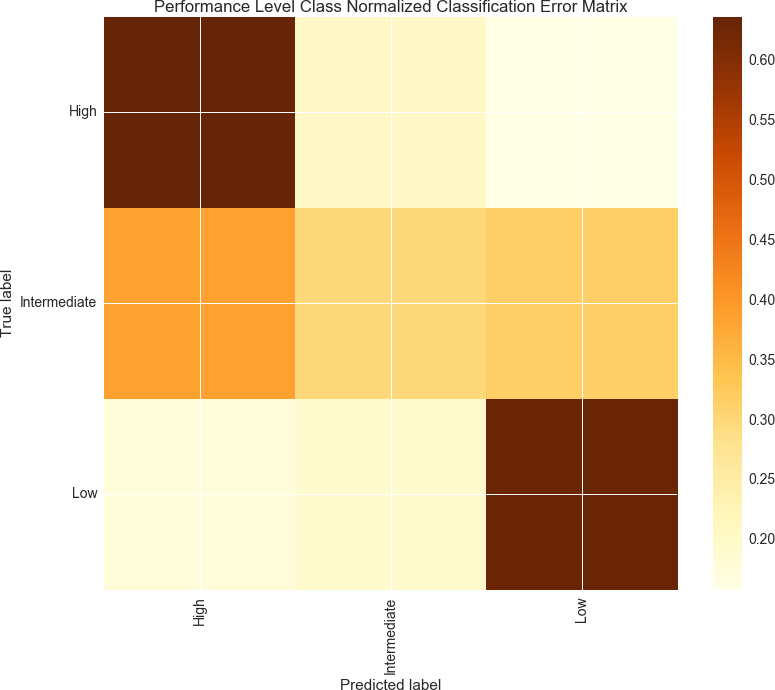
\includegraphics[width=1\columnwidth]{figures/ConfusionMatrixPerformanceLevelClass/ConfusionMatrixPerformanceLevelClass}
\caption{{Classification error matrix for prediction of performance class using a random forest model
\label{fig:performance_classification}%
}}
\end{center}
\end{figure}

Figure \ref{sec:featureimportance_performclass} shows the variable importance calculation as it relates to classification for all three classes. The top features for this model are a mix of statistical features and model-based features. Within the statistical features category, the seasonal range for both winter and summer are top features in addition to several daily ratios. For model-based features, the loadshape model errors, the \emph{stl} model residuals, and the eemeter residuals are all present.

\begin{figure}[ht!]
\begin{center}
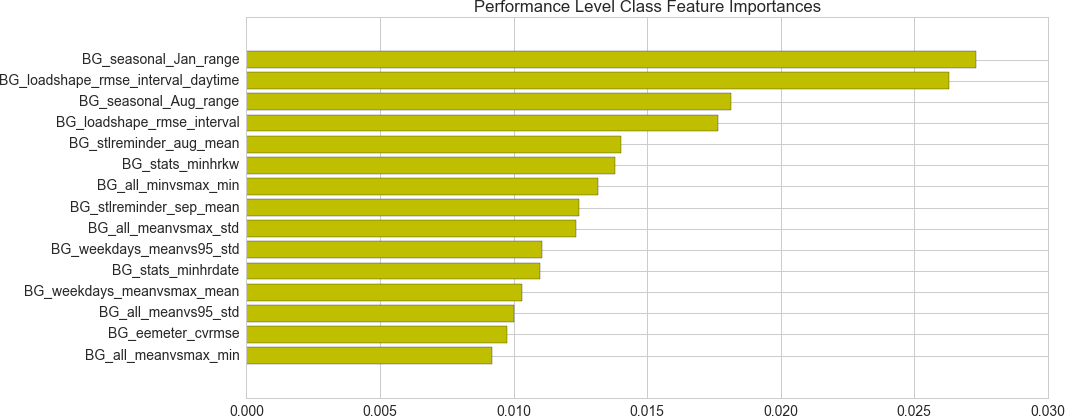
\includegraphics[width=1\columnwidth]{figures/FeatureImportancePerformanceLevelClass/FeatureImportancePerformanceLevelClass}
\caption{{Importance of features according to random forest model in prediction of building performance class
\label{sec:featureimportance_performclass}%
}}
\end{center}
\end{figure}

\subsection{High versus Low Consumption Comparison}
\label{sec:highvslow}

The two classifications chosen for this objective are intuitively the \emph{high} and \emph{low} consuming buildings. This part of the analysis gives a more in-depth perspective of exactly which features are most important in the differentiation between these two types of buildings. This understanding provides insight on potentially what behavior in a building results in good or poor performing buildings. Once again, the highly comparative time-series analysis (hctsa) code repository is used for this process. Figure \ref{fig:featurecluserting_performanceclass} is a correlation matrix showing the top forty features as determined by hctsa according to the in-sample linear classification performance. Eight clusters of features are detected on discriminating between high and low consumption. The first set of correlated features seen in the upper left corner of the figure contains a mix of statistical and daily pattern-based features. The second cluster includes a set of four features related to daily ratios. The third and largest group is mostly statistical and daily ratio-based features. The fourth, sixth, seventh, and eighth clusters all contain mostly in-class similarity and temporal features created using \emph{jmotif}. These features are an indicator of how well a building's patterns fit within its own class. An interesting aspect of these features is their lack of correlation with the rest of the larger set. This situation indicates that they are capturing unique behavior, not picked up by others in the set. These clusters are also relatively small with only one to four members. The sixth cluster contains a set of features that are mostly generated by the \emph{stl} decomposition models.

\begin{figure}[ht!]
\begin{center}
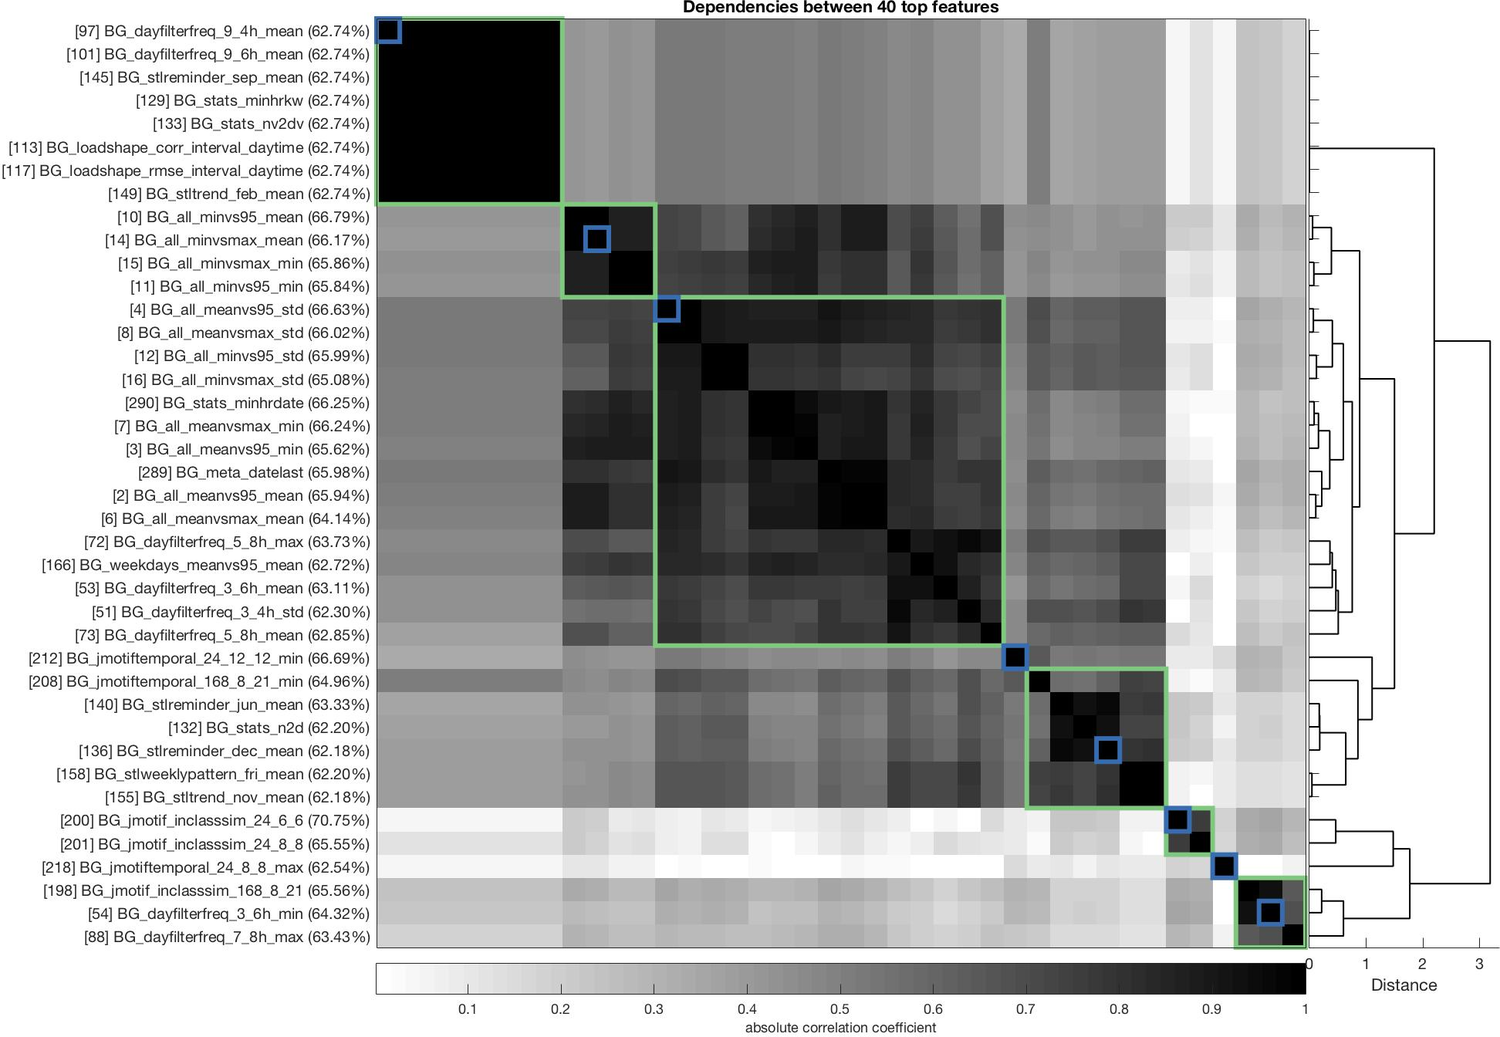
\includegraphics[width=1\columnwidth]{figures/Output_HighvsLow_Top40/Output_HighvsLow_Top40}
\caption{{Clustering of dominant features in the comparison of high and low consumption performance classes
\label{fig:featurecluserting_performanceclass}%
}}
\end{center}
\end{figure}

Figure \ref{fig:topfivefeatures_highvslow} shows the probability distributions of the top five performing features in predicting high versus low consumption. The number one top feature for differentiating between these classes is the daily in-class similarity feature that is generated by the \emph{jmotif} process. This feature informs us that buildings from all classes that have the highest average daily pattern similarity to their peers are often also amongst the highest consuming buildings in their class. Buildings that are on average less similar in their daily patterns to their class are often in a lower percentile of consumption. This fact suggests that many buildings that are misclassified are lower consumers of electricity. The second and fourth features are daily statistical ratios. Buildings with higher consumption tend to have more \emph{flat} profiles, likely due to a higher base load during unoccupied periods. The third top classifier is also created using the \emph{jmotif} library and it suggests that a building that whose minimum daily pattern specificity across the year is an indicator of higher than average consumption. 

\begin{figure}[ht!]
\begin{center}
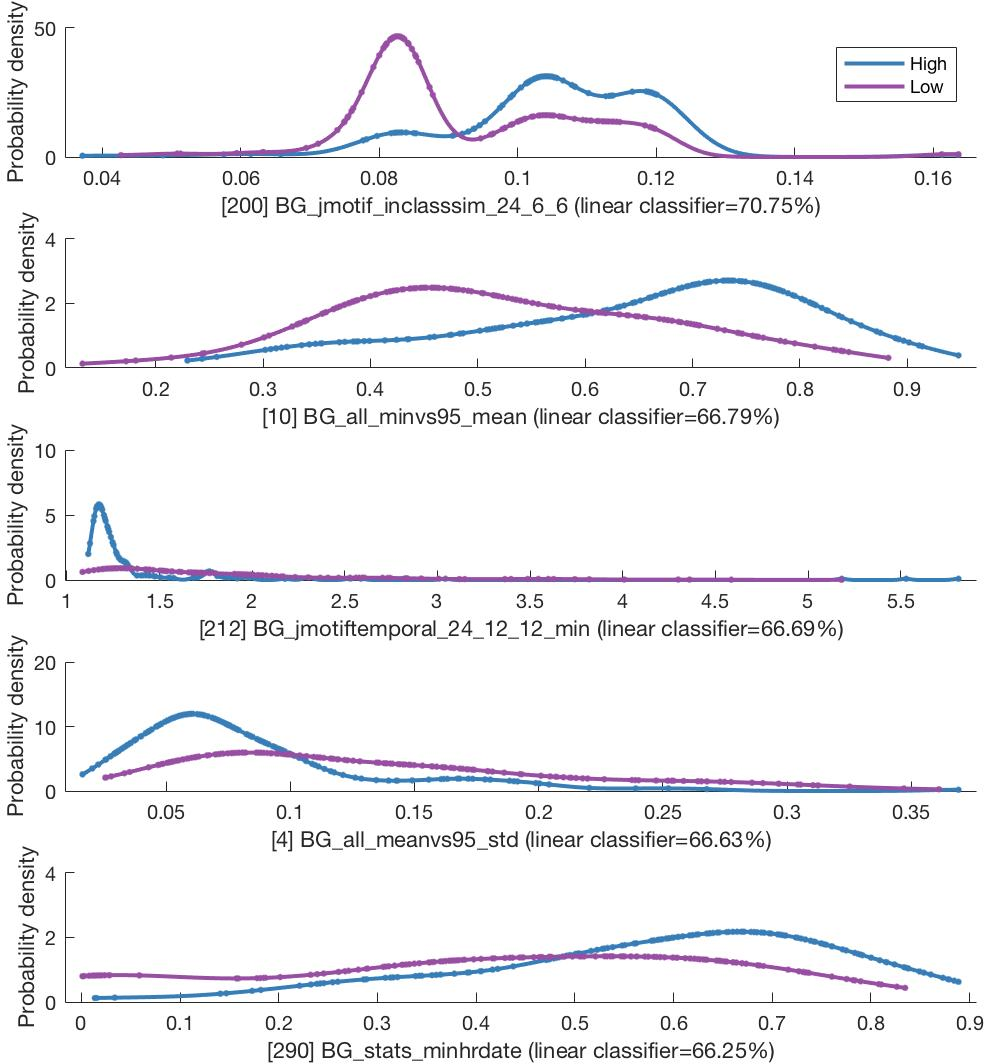
\includegraphics[width=0.7\columnwidth]{figures/Output_HighvsLow_Features_1-5/Output_HighvsLow_Features_1-5}
\caption{{Probability density distribution of top five features in characterizing the difference between high and low consumption
\label{fig:topfivefeatures_highvslow}%
}}
\end{center}
\end{figure}

Figure \ref{sec:highvslow_nullhypth} shows the probability distribution of the features in their ability to distinguish between high and low consumption as compared to a baseline. The mean of the created features is approximately 58\%, while the null mean is 51\%. This situation indicates that the generated temporal features have a significant impact on the prediction and evaluation of whether a building performs well or not.

\begin{figure}[ht!]
\begin{center}
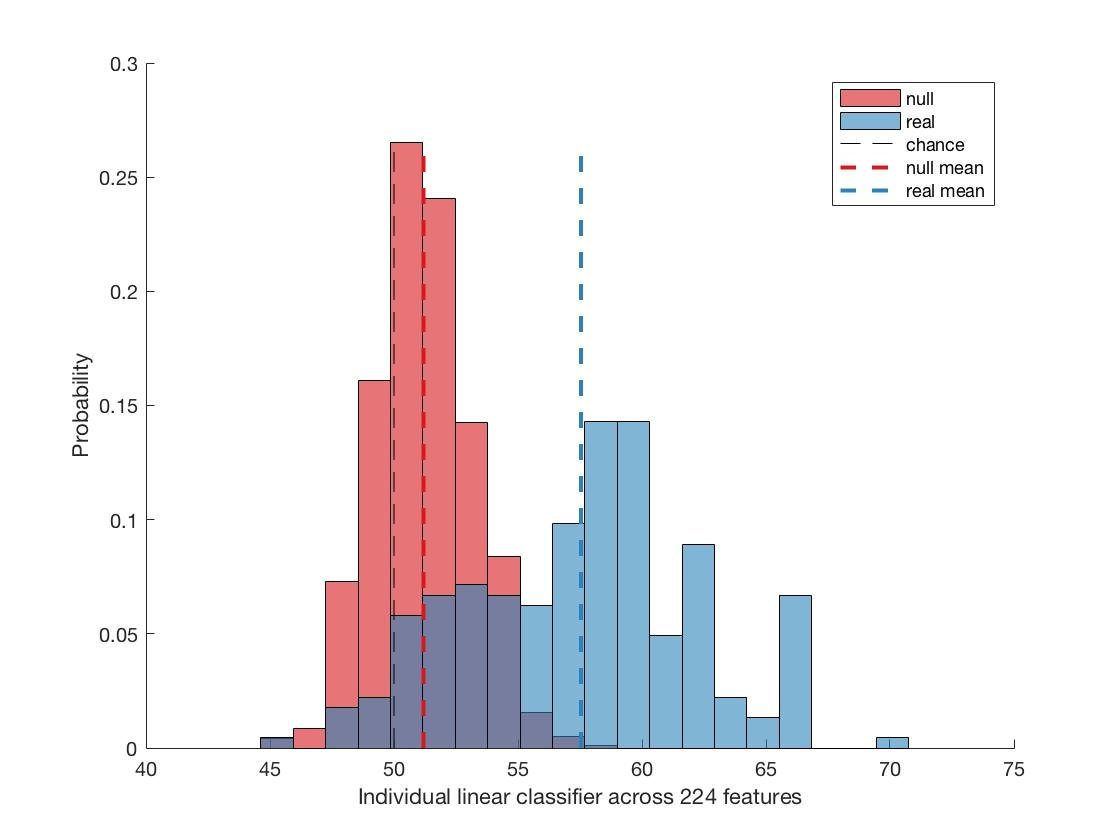
\includegraphics[width=0.7\columnwidth]{figures/Output_HighvsLow_Dist/Output_HighvsLow_Dist}
\caption{{Ability of temporal features to distinguish between high and low consumers as compared to the null hypothesis
\label{sec:highvslow_nullhypth}%
}}
\end{center}
\end{figure}

\subsection{Discussion with Campus Case Study Subjects}
\label{sec:performanceclass_oncasestudy}

In a situation similar to the discussion about building use type, participants in the case studies were guided through the process of analysis using a subset of features from buildings on their campus. Figure \ref{fig:breakdown_performanceclass} illustrates a graphic that was shown to the groups. In this case, the buildings are divided into two classes: \emph{Good} and \emph{Bad}. These categories are based on whether the building falls in the upper or lower 50\% within its class. The first observation by the case study participants is that the load diversity, or the daily maximum versus minimum, is a strong indicator of the performance class. This fact is not surprising as this metric indicates the magnitude of the base load consumption as compared to the peak. Other relatively strong differentiators, in this case, are cooling energy, seasonal changes, and weekly specificity. The discussions related to this graphic centered around the potential for the temporal features to inform \emph{why} a building is performing well or not. The results of Section \ref{sec:highvslow} also include such clues on why a building may be in a high or low performing state. 

\begin{figure}[ht!]
\begin{center}
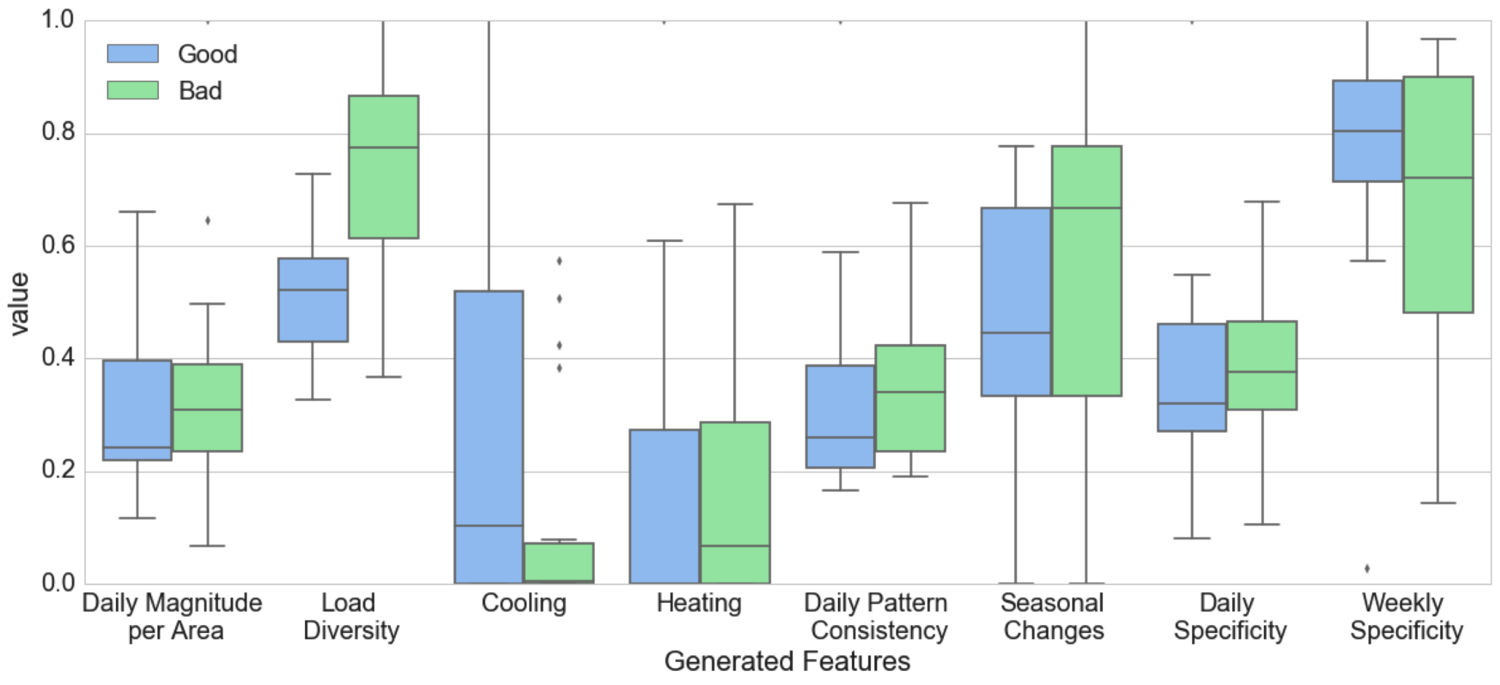
\includegraphics[width=0.98\columnwidth]{figures/consumptionbreakdown/consumptionbreakdown}
\caption{{Simplified breakdowns of general features according to performance level that were presented to case study subjects
\label{fig:breakdown_performanceclass}%
}}
\end{center}
\end{figure}

Figure \ref{fig:campusperformance} illustrates another graphic related to building consumption classes that were discussed with case study participants. This graphic is an overview of the distributions of the simplified set of features for a certain campus as compared to the entire set of case study buildings. This graphic shows where the buildings on this campus stand as compared to their peers. In this case, the buildings are on the higher end of the normalized consumption, which could likely be because they're also almost all in the highest 20\% of buildings for heating energy consumption. The buildings also have a relatively high load diversity, thus the base loads for this campus are likely higher than average and interventions could be designed to reduce this unoccupied load. Many of the case study participants saw this insight as useful as it \emph{supplements} the information from benchmarking.

\begin{figure}[ht!]
\begin{center}
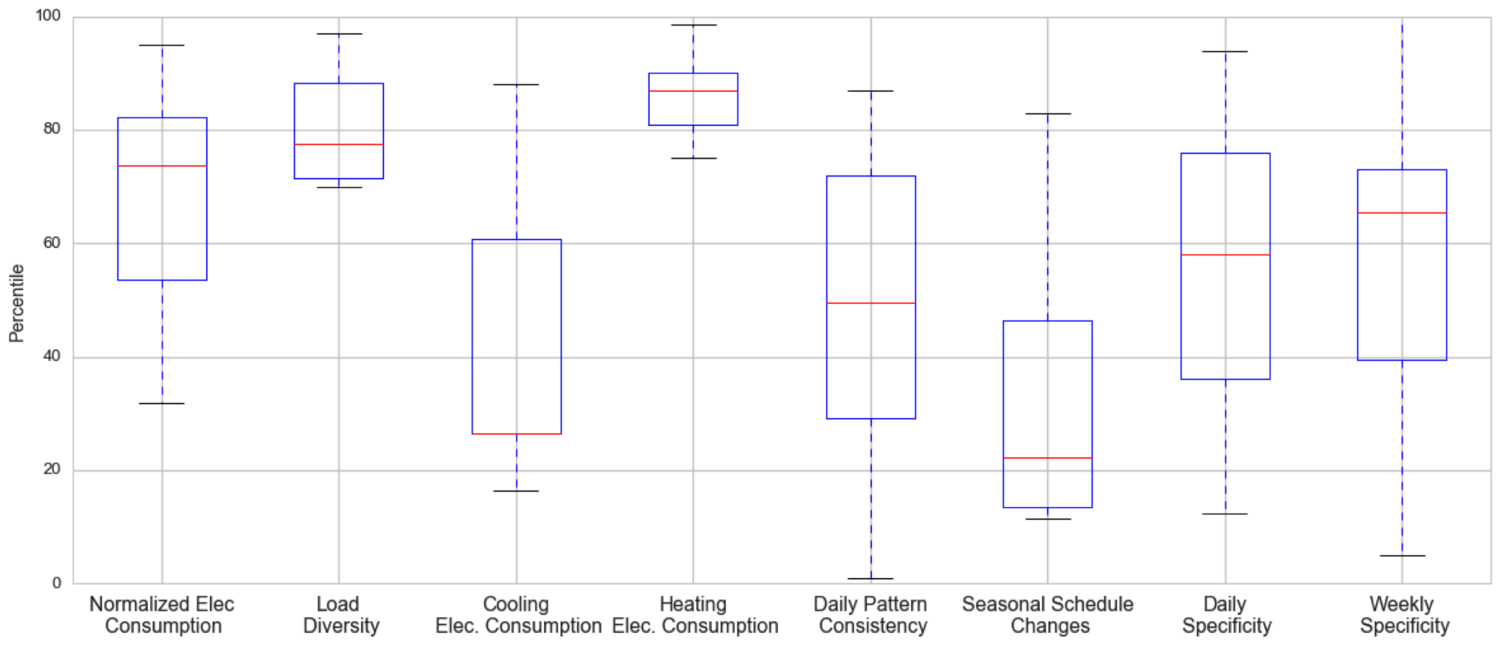
\includegraphics[width=0.98\columnwidth]{figures/benchmarkingbuildings/benchmarkingbuildings}
\caption{{Feature distributions of a single campus as compare to all other case study buildings
\label{fig:campusperformance}%
}}
\end{center}
\end{figure}

\section{Characterization of Operations Strategies}
\label{sec:operations_strategies}

The final characterization objective for the case studies is the ability for the temporal features to classify buildings from the same campus, and thus buildings that are being operated in similar ways. This characterization takes to into account the similarity in occupancy schedules, patterns of use, and other factors related to how a building operates. Like the performance classes, this type of classification is more important in understanding the features that contribute to the differentiation, rather than the classification itself. Seven campuses were selected from the 507 buildings to create seven \emph{groups} of buildings to characterize the difference between their operating behavior. Features were removed for this objective that are indicators of weather sensitivity as these would be related to the location of the buildings, and thus, the campus that they're located. Figure \ref{fig:operations_classification} illustrates the results from the random forest model trained on these data. The accuracy of this model is 80.5\% as compared to a baseline of 16.9\%. The model is excellent at predicting some of the groups, such as groups 1-4, which more deficient in others, such as 5-7. The high accuracy of this prediction is surprising and lends itself to the ability of the temporal features and the random forest model to predict the operational normalities of these buildings.

\begin{figure}[ht!]
\begin{center}
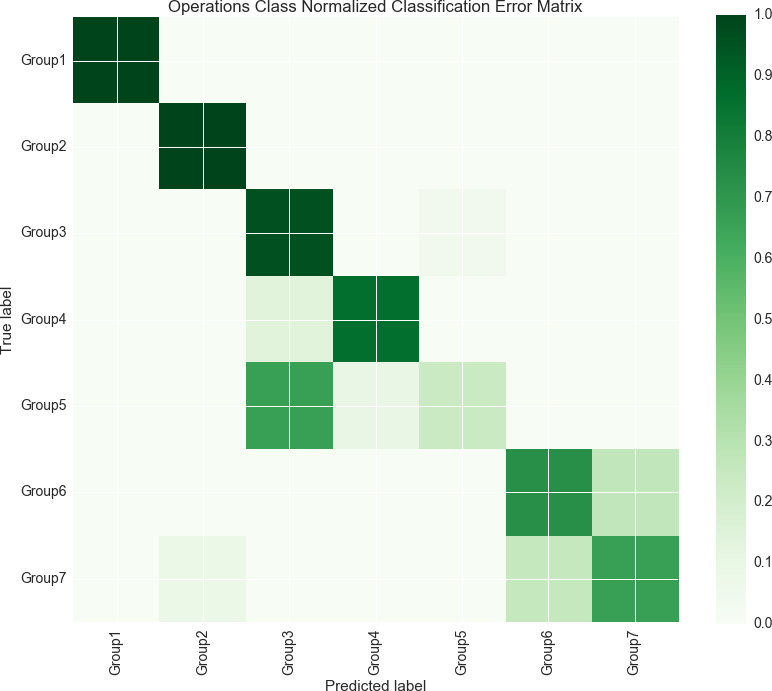
\includegraphics[width=1\columnwidth]{figures/ConfusionMatrixOperationsClass/ConfusionMatrixOperationsClass}
\caption{{Classification error matrix for prediction of operations group type using a random forest model
\label{fig:operations_classification}%
}}
\end{center}
\end{figure}

Figure \ref{sec:featureimportance_operations} illustrates the temporal features identified by the random forest model as the most important in class differentiation. One can observe several daily pattern-based features in addition to statistical and daily ratio-based features. This finding lends weight to the assumption that similarity in daily scheduling is a key discriminator between the operations of various campuses.

\begin{figure}[ht!]
\begin{center}
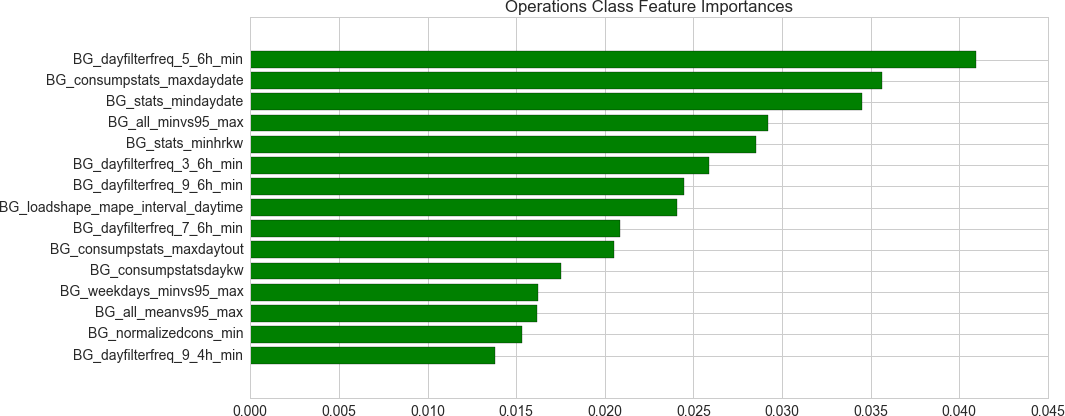
\includegraphics[width=1\columnwidth]{figures/FeatureImportanceOperationsClass/FeatureImportanceOperationsClass}
\caption{{Importance of features in prediction of operations type
\label{sec:featureimportance_operations}%
}}
\end{center}
\end{figure}

\subsection{Group 1 versus Group 2 Comparison}
\label{sec:group1vsgroup2}

Groups 1 and 2 were selected to undertake a deeper analysis using the highly comparative time-series analysis library. Figure \ref{fig:featurecluserting_operationsgroups} shows the top forty features and their correlated clusters. The first and largest cluster of features, in this case, are from the breakout detection process, a calculation of long-term volatility. This insight suggests that breakouts are a key discriminatory aspect of seasonal patterns that would exist for buildings being operated in the same way. The third cluster includes a diverse set of features including a few from the loadshape library and several statistics-based metrics. The fourth cluster contains features from the jmotif library, including both in-class similarity and specificity metrics. The remaining clusters are all quite small, only containing one or two features, and are made up of both pattern and motif-based features.

\begin{figure}[ht!]
\begin{center}
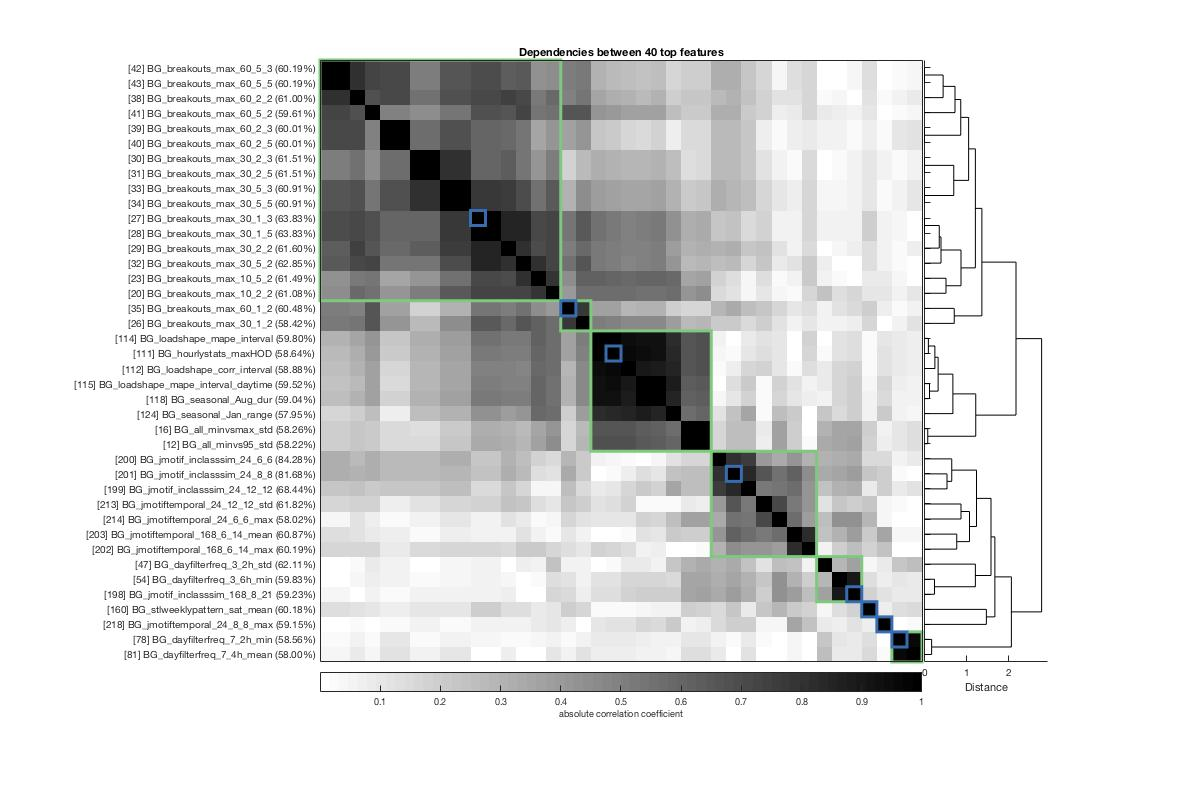
\includegraphics[width=1\columnwidth]{figures/Output_Group1vsGroup2_Top40/Output_Group1vsGroup2_Top40}
\caption{{Clustering of dominant features in the comparison of operations group 1 and 2
\label{fig:featurecluserting_operationsgroups}%
}}
\end{center}
\end{figure}

Figure \ref{fig:topfivefeatures_operationsclass} illustrates the top five features in the comparison of Group 1 and 2. The first three features are variations of in-class similarity. This indication shows that the buildings from these two particular groups are differentiated by how much the buildings fit within their designated class. The fourth and fifth dominant features are associated with the number of breakouts and long-term volatility.

\begin{figure}[ht!]
\begin{center}
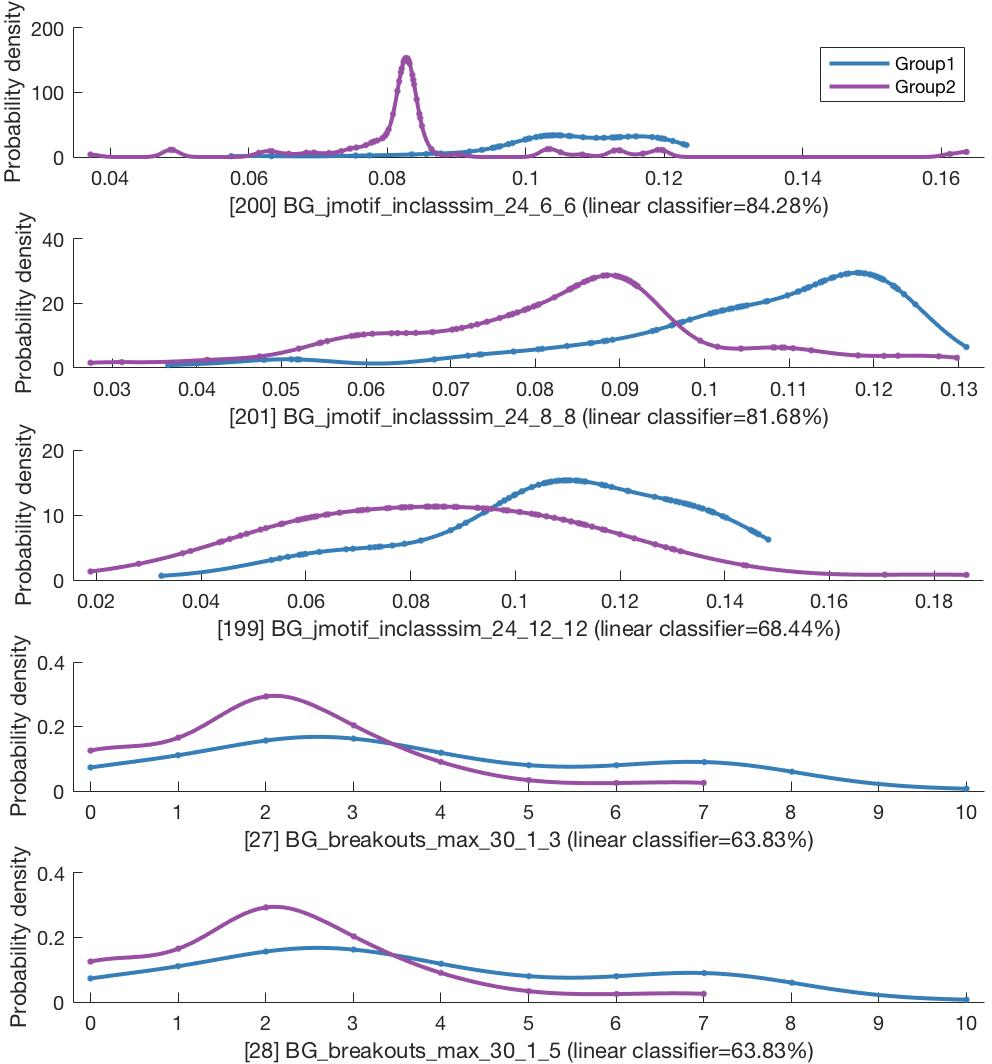
\includegraphics[width=0.7\columnwidth]{figures/Output_Group1vsGroup2_Features_1-5/Output_Group1vsGroup2_Features_1-5}
\caption{{Probability density distribution of top five features in characterizing the difference between Group 1 and 2 operations classes
\label{fig:topfivefeatures_operationsclass}%
}}
\end{center}
\end{figure}

Figure \ref{sec:operationstypes_nullhypth} illustrates how well all of the features can discriminate the difference between these two groups of buildings. The separation for a majority of the features is not much greater than the null mean, but the top differentiators are quite prominent.

\begin{figure}[ht!]
\begin{center}
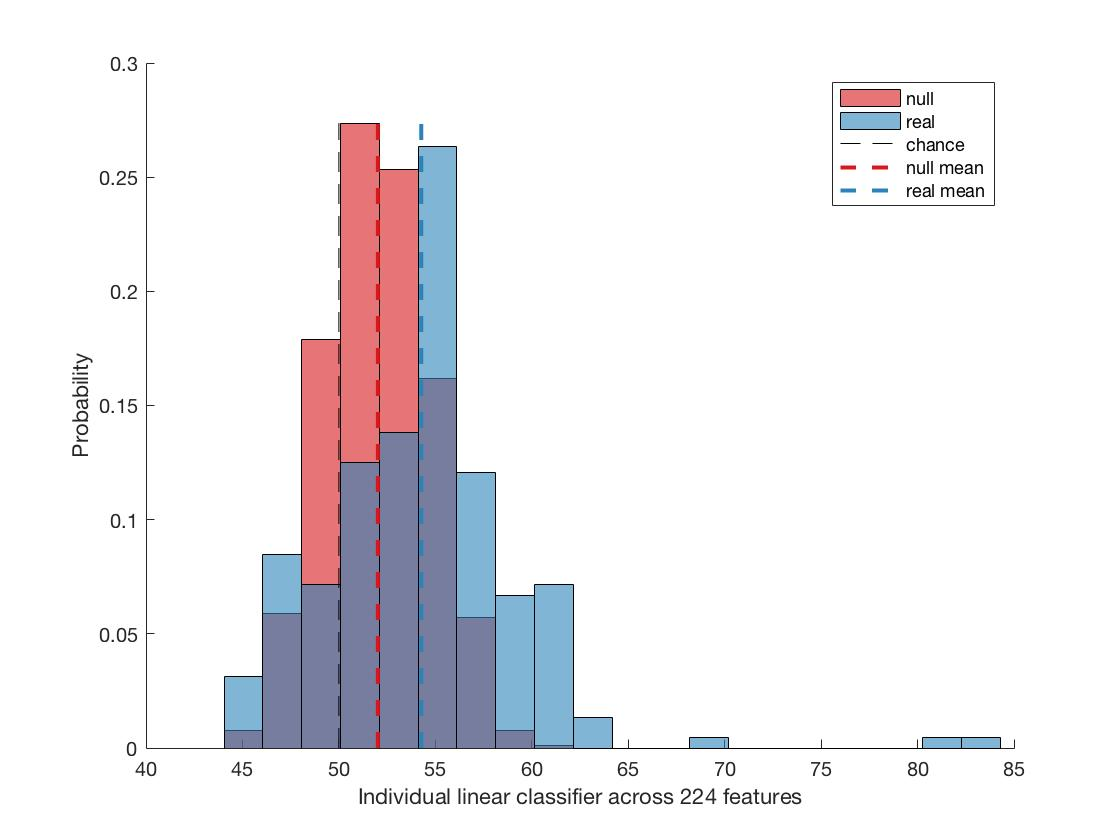
\includegraphics[width=0.7\columnwidth]{figures/Output_Group1vsGroup2_Dist/Output_Group1vsGroup2_Dist}
\caption{{Ability of temporal features to distinguish between group 1 and 2 operations types as compared to the null hypothesis
\label{sec:operationstypes_nullhypth}%
}}
\end{center}
\end{figure}

% \section{Overview of Temporal Features Influence on Objectives}
% \label{sec:overviewuroftemporalfeat}

% This final subsection aggregates the variable importance from all three random forest models from Sections \ref{sec:buildinguse}-\ref{sec:operations_strategies} and discusses the overlap and complementary nature. 

% The development of the features in this study was completed with the intent of capturing much of the common building performance characterization techniques commonly found in the research literature. Additionally, several novel pattern-based techniques were implemented and tested. It is of interest to test this features set against a benchmark set of temporal data mining techniques to understand how thorough the proposed set of metrics are at characterizing the data. This benchmark comparison is done using the \emph{highly comparative time-series analysis} feature library \cite{Fulcher_2013}. This library includes over 9000 temporal features covering a vast range of algorithm types.

% %data for the following table is from: http://rsif.royalsocietypublishing.org/content/royinterface/suppl/2013/04/03/rsif.2013.0048.DC1/rsif20130048supp2.pdf

% \begin{table} 
%     \begin{tabular}{ c c c }
%         \textbf{Feature Category} & \textbf{Brief Description} & \textbf{Number of Features} \\
%         Test & Test & Test \\ 
%         Test &  &  \\ 
%          &  &  \\ 
%          &  &  \\ 
%          &  &  \\ 
%          &  &  \\ 
%          &  &  \\ 
%          &  &  \\ 
%          &  &  \\ 
%          &  &  \\ 
%          &  &  \\ 
%     \end{tabular} 
% \end{table}
